\documentclass[UTF8,a4paper,10pt,nocolorlinks]{ctexart}
\usepackage[left=2.50cm, right=2.50cm, top=2.50cm, bottom=2.50cm]{geometry} %页边距
\CTEXsetup[format={\Large\bfseries}]{section} %设置章标题居左   
\usepackage{ctex}
\CTEXoptions[today=old]
\usepackage{cite}
\usepackage{textcomp}
\usepackage{listings}
\usepackage{xcolor}
\usepackage{varioref}
\usepackage{ctex}
\usepackage{multicol}
\usepackage{amssymb} 
\usepackage{setspace}
\usepackage{tikz} 
\usepackage{mdframed}
\usepackage{titletoc}
\usepackage{etoolbox}

\usepackage{helvet}
\usepackage{caption}
\usepackage{multicol} 
\usepackage{changepage}
\usepackage{graphics}
\usepackage{amsmath, amsfonts, amssymb}
\usepackage[english]{babel}
\usepackage{color}      
\usepackage{graphicx}   
\usepackage{url}        
\usepackage{bm}         
\usepackage{multirow}
\usepackage{booktabs}
\usepackage{epstopdf}
\usepackage{epsfig}
\usepackage{algorithm}
\usepackage{algorithmic}

\usepackage[pagestyles]{titlesec}
\renewcommand{\algorithmicensure}{ \textbf{Input:}} 
\renewcommand{\figurename}{图}
\newcommand{\upcite}[1]{\textsuperscript{\textsuperscript{\cite{#1}}}}

\newpagestyle{teststyle}{
  \sethead{\emph{姓名:冯学伟}}{\emph{\sectiontitle}}{\emph{第\thepage页}}
  \renewcommand{\makeheadrule}{
    \makebox[0pt][l]{\rule[-.3\baselineskip]{\linewidth}{.5pt}}
    \rule[-.4\baselineskip]{\linewidth}{.5pt}
  }
}
\usepackage{color}
\usepackage{subfigure}
\usepackage{changepage}
\usepackage{fancyhdr} %设置页眉、页脚
\pagestyle{fancy}  %%%单线页眉
\fancyhead{}
\fancyhead[LO]{基于视觉的固定翼小型无人机自主降落技术研究}
\fancyhead[RO]{冯学伟}
\fancypagestyle{plain}{
  \pagestyle{fancy}
}
\usepackage{shorttoc}
\usepackage{xcolor}
\usepackage{mdframed}
\usepackage{titletoc}

\DeclareRobustCommand{\chuhao}{\fontsize{42pt}{\baselineskip}\selectfont}  % 初号
\DeclareRobustCommand{\xiaochu}{\fontsize{36pt}{\baselineskip}\selectfont} % 小初
\DeclareRobustCommand{\yihao}{\fontsize{26pt}{\baselineskip}\selectfont}   % 一号
\DeclareRobustCommand{\xiaoyi}{\fontsize{24pt}{\baselineskip}\selectfont}  % 小一
\DeclareRobustCommand{\erhao}{\fontsize{22pt}{\baselineskip}\selectfont}   % 二号
\DeclareRobustCommand{\xiaoer}{\fontsize{18pt}{\baselineskip}\selectfont}  % 小二
\DeclareRobustCommand{\sanhao}{\fontsize{16pt}{\baselineskip}\selectfont}  % 三号 
\DeclareRobustCommand{\xiaosan}{\fontsize{15pt}{\baselineskip}\selectfont} % 小三
\DeclareRobustCommand{\sihao}{\fontsize{14pt}{\baselineskip}\selectfont}   % 四号
\DeclareRobustCommand{\xiaosi}{\fontsize{12pt}{\baselineskip}\selectfont}  % 小四
\DeclareRobustCommand{\wuhao}{\fontsize{10.5pt}{\baselineskip}\selectfont} % 五号
\DeclareRobustCommand{\xiaowu}{\fontsize{9pt}{\baselineskip}\selectfont}   % 小五
\DeclareRobustCommand{\liuhao}{\fontsize{7.5pt}{\baselineskip}\selectfont} % 六号
\DeclareRobustCommand{\xiaoliu}{\fontsize{6.5pt}{\baselineskip}\selectfont}% 小六
\DeclareRobustCommand{\qihao}{\fontsize{5.5pt}{\baselineskip}\selectfont}  % 七号

\lstset{numbers=left,numberstyle=\tiny,
breaklines=true,  %代码过长则换行
keywordstyle=\color{blue!70},commentstyle=\color{red!50!green!50!blue!50},frame=shadowbox, rulesepcolor=\color{gray!20!green!20!blue!20},escapeinside=``,xleftmargin=2em,xrightmargin=2em, aboveskip=1em}

\providecommand{\keywords}[1]{\textbf{\textit{keywords---}} #1}

 
\usepackage{hyperref} %bookmarks
% \usepackage[colorlinks,linkcolor=red,anchorcolor=blue,citecolor=green,CJKbookmarks=True]{hyperref}
\hypersetup{colorlinks, bookmarks, unicode} % unicode
 
\captionsetup[figure]{labelfont={bf},labelformat={default},labelsep=period,name={图}}
\newenvironment{figurehere}
{\def\@captype{figure}}
{}

\title{
    \huge{\textbf{基于视觉的固定翼小型无人机自主降落技术研究}}\\
    \Large{\textbf{Research on Autonomous Landing Technology of fixed Wings Small Unmanned  Aerial Vehicle Based on Vision}}
}

\author{冯学伟}
\date{\today}

\begin{document}
    % \maketitle
    % \chapter{title}
\begin{center}
    \begin{center} % 选择一种技术进行研究
        \huge{\textbf{基于视觉的固定翼小型无人机自主降落技术研究}}\\
        \emph{\Large{\textbf{
            Research on Autonomous Landing Technology of fixed Wings Small Unmanned Aerial Vehicle Based on Vision
        }}}\\     
    \end{center}
\end{center}
    \chapter{abstract}
\begin{adjustwidth}{0cm}{0cm}
    \emph{\textbf{摘\hspace{0.5em}要:} 以固定翼小型无人机的自主着陆控制为研究背景,提出了一种基于光流的固定翼小型无人机在移动降落架上的自主着
    陆控制方法。该方法首先\dots\dots; 其次\dots \dots; 最后在 simulink 环境下搭建动态仿真系统,仿真
    结果表明,使用本文方法可以有效实现飞行器的自主着陆控制. 
    % 在最后就机器学习在计算机视觉中的应用前景进行了展望。随机森林是近几年非常热门的分类方法,由于其训练和测试速度快,被许多学者用于图像匹配、动作识别等领域。利用在线的随机森林,能对跟踪目标进行不断学习,以获取目标最新的外观特征,从而及时完善跟踪,以达到最佳的状态。
    }
    \begin{flushleft}
    \emph{{\textbf{关键字:}} 固定翼小型无人机; 计算机视觉; 自主降落; 目标追踪; 光流}
    \end{flushleft}
\end{adjustwidth}
\begin{adjustwidth}{0cm}{0cm}
    \emph{\textbf{Abstract:}
    Taking the autonomous landing control of fixed-wing small unmanned aerial vehicles as the research background, 
    a method of autonomous landing control of fixed-wing small unmanned aerial vehicles based on optical flow is proposed. 
    This method, first of all, is \dots \dots, and \dots \dots, then uses the runway line as a feature to calculate its sparse linear optical flow field and combines The camera model and the relationship between the optical flow field and the velocity field use the horizontal flow of the runway line as system feedback to design the control system. Finally, a dynamic simulation system is built under the simulink environment. The simulation results show that the method of this paper can effectively achieve the autonomous landing control of the aircraft.}\par
\end{adjustwidth}
\begin{keywords}
    \emph{\noindent fixed-wing, Computer Vision, Autonomous landing, Target Tracking, light flow}
\end{keywords}
    \setcounter{page}{1}        %从下面开始编页,页脚格式为导言部分设置的格式

    \pagestyle{teststyle}

    \chapter{introduce}
\section{引言}
        \begin{itemize}
            \item 本课题研究背景
            \item 本课题研究前景
            \item 本课题知识难点
            \item 本课题结构罗列
        \end{itemize}
    \chapter{controllers}
\section{无人机控制器}
无人机总的概述 \dots.
\begin{itemize}
    \item 无人机三大控制器介绍
    \item 无人机内部控制器数据流走向
\end{itemize}
        \chapter{landingLogical}
    \section{飞行器着陆原理分析}   
    通常的基础方法,      
    \begin{itemize}
        \item 光流场, 三个阶段
        \item 横向控制
        \item 纵向控制
    \end{itemize}
        \chapter{visionGuidence}
    
    \section{无人机视觉引导}
        \subsection{视觉体系结构}
            \begin{itemize}
                \item 视觉体系结构阐述
                \item 视觉数据流走向
            \end{itemize}
    % 前面的都是基础知识, 方法, 只是介绍, 以及各自的优点和缺点, 我需要解决的问题, 每一章都说一个缺点, 在后面 针对上面的缺点进行解决

        \chapter{visionGuidence}
    
    \section{融合}
    若内容太多, 继续拆分 \\
    数学模式 方法 公式推导, 可以对应的说(分节), 也可以整合到一起, 看内容的多少
    \par 传感器选择
    \par 横向控制
    \par 纵向控制
    \par 引导算法
        \chapter{simulations}
    
    \section{仿真平台的搭建}
        
        这个不太了解\dots.
        
        目前还是需要多看, 多了解. 
    \documentclass[UTF8,a4paper,10pt,nocolorlinks]{ctexart}
\usepackage[left=2.50cm, right=2.50cm, top=2.50cm, bottom=2.50cm]{geometry} %页边距
\CTEXsetup[format={\Large\bfseries}]{section} %设置章标题居左   
\usepackage{ctex}
\CTEXoptions[today=old]
\usepackage{cite}
% 代码块儿
\usepackage{textcomp} % 必须加上,否则报错
\usepackage{listings}
\usepackage{xcolor}
% \usepackage{fontspec}
% \setmonofont{Consolas}
\usepackage{varioref}       % ref 跨页调用
\usepackage{ctex}
\usepackage{multicol}
\usepackage{amssymb}        % 等于号 上面 加一个三角形
\usepackage{setspace}
\usepackage{tikz} % package used for the tikz
\usepackage{mdframed}
\usepackage{titletoc}
\usepackage{etoolbox}

\usepackage{helvet}
\usepackage{caption}
\usepackage{multicol} %用于实现在同一页中实现不同的分栏
\usepackage{changepage}
\usepackage{graphics}
\usepackage{amsmath, amsfonts, amssymb} % math equations, symbols
\usepackage[english]{babel}
\usepackage{color}      % color content
\usepackage{graphicx}   % import figures
\usepackage{url}        % hyperlinks
\usepackage{bm}         % bold type for equations
\usepackage{multirow}
\usepackage{booktabs}
\usepackage{epstopdf}
\usepackage{epsfig}
\usepackage{algorithm}
\usepackage{algorithmic}

\usepackage[pagestyles]{titlesec}
% \renewcommand{\algorithmicrequire}{ \textbf{Input:}}     % use Input in the format of Algorithm  
% \renewcommand{\algorithmicinput}{ \textbf{Input:}}     % use Input in the format of Algorithm  
\renewcommand{\algorithmicensure}{ \textbf{Input:}} % use Initialize in the format of Algorithm  
% \renewcommand{\algorithmicreturn}{ \textbf{Output:}}     % use Output in the format of Algorithm  
\renewcommand{\figurename}{图}
% 引用参考文献标号显示在右上角
\newcommand{\upcite}[1]{\textsuperscript{\textsuperscript{\cite{#1}}}}

\newpagestyle{teststyle}{
  \sethead{学号: 2019520941}{\sectiontitle}{第\thepage页}
  \renewcommand{\makeheadrule}{
    \makebox[0pt][l]{\rule[-.3\baselineskip]{\linewidth}{.5pt}}
    \rule[-.4\baselineskip]{\linewidth}{.5pt}
  }
}
\usepackage{color}
\usepackage{subfigure}
\usepackage{changepage}
\usepackage{fancyhdr} %设置页眉、页脚
\pagestyle{fancy}  %%%单线页眉
\fancyhead{}
\fancyhead[LO]{学习总结}
\fancyhead[RO]{冯学伟}
% \fancyfoot[RO]{\thepage}
\fancypagestyle{plain}{%
  \pagestyle{fancy}
}
\usepackage{shorttoc}
\usepackage{xcolor}
\usepackage{mdframed}
\usepackage{titletoc}
% \renewcommand{\today}{\CJKnumber\year 年 \CJKnumber\month 月 \CJKnumber\day 日}

\DeclareRobustCommand{\chuhao}{\fontsize{42pt}{\baselineskip}\selectfont}  % 初号
\DeclareRobustCommand{\xiaochu}{\fontsize{36pt}{\baselineskip}\selectfont} % 小初
\DeclareRobustCommand{\yihao}{\fontsize{26pt}{\baselineskip}\selectfont}   % 一号
\DeclareRobustCommand{\xiaoyi}{\fontsize{24pt}{\baselineskip}\selectfont}  % 小一
\DeclareRobustCommand{\erhao}{\fontsize{22pt}{\baselineskip}\selectfont}   % 二号
\DeclareRobustCommand{\xiaoer}{\fontsize{18pt}{\baselineskip}\selectfont}  % 小二
\DeclareRobustCommand{\sanhao}{\fontsize{16pt}{\baselineskip}\selectfont}  % 三号 
\DeclareRobustCommand{\xiaosan}{\fontsize{15pt}{\baselineskip}\selectfont} % 小三
\DeclareRobustCommand{\sihao}{\fontsize{14pt}{\baselineskip}\selectfont}   % 四号
\DeclareRobustCommand{\xiaosi}{\fontsize{12pt}{\baselineskip}\selectfont}  % 小四
\DeclareRobustCommand{\wuhao}{\fontsize{10.5pt}{\baselineskip}\selectfont} % 五号
\DeclareRobustCommand{\xiaowu}{\fontsize{9pt}{\baselineskip}\selectfont}   % 小五
\DeclareRobustCommand{\liuhao}{\fontsize{7.5pt}{\baselineskip}\selectfont} % 六号
\DeclareRobustCommand{\xiaoliu}{\fontsize{6.5pt}{\baselineskip}\selectfont}% 小六
\DeclareRobustCommand{\qihao}{\fontsize{5.5pt}{\baselineskip}\selectfont}  % 七号

\lstset{numbers=left,numberstyle=\tiny,
breaklines=true,  %代码过长则换行
keywordstyle=\color{blue!70},commentstyle=\color{red!50!green!50!blue!50},frame=shadowbox, rulesepcolor=\color{gray!20!green!20!blue!20},escapeinside=``,xleftmargin=2em,xrightmargin=2em, aboveskip=1em}

\providecommand{\keywords}[1]{\textbf{\textit{keywords---}} #1}

 
\usepackage{hyperref} %bookmarks
% \usepackage[colorlinks,linkcolor=red,anchorcolor=blue,citecolor=green,CJKbookmarks=True]{hyperref}
\hypersetup{colorlinks, bookmarks, unicode} % unicode
 
\captionsetup[figure]{labelfont={bf},labelformat={default},labelsep=period,name={图}}
\newenvironment{figurehere}
{\def\@captype{figure}}
{}

\title{
    \huge{\textbf{2020.07.07 第一次总结}}\\
}
\author{冯学伟}
\date{2020.07.07}

\begin{document}
    \maketitle
    % \renewcommand{\contentsname}{目录}  % 将Contents改为目录
    % \tableofcontents
    % \thispagestyle{empty} % 设置当前页 页版式
    
   
    本周计划: 
    \begin{itemize}
      \item 理论学习: 继续就那本书进行学习, 按照进度, 应该可以看一章多一点.
      \item 调bug: 将HITL调通
    \end{itemize}
    % \section{本周的学习总结}
    %     \subsection{chapter 3}
    %     本章, 主要介绍了刚体运动的运动学(kinematics)和动力学(dynamics); 其中主要定义了
    %     \begin{itemize}
    %       \item 位置和速度的关系(kinematics)
    %       \item 动力学表达式
    %       \item 12个状态量的表达式
    %     \end{itemize}
    %     首先介绍了\textcolor{red}{声明了MAV状态变量}, 12个, 
    %     其中, 和平移运动相关的三个位置变量(ned), 
    %     三个速度变量($u, v, \omega$, $i^{b}, j^{b}, k^{b}$), 
    %     三个角度(roll($F^{v2}$), pitch($F^{v1}$), yaw($F^{v}$)), 
    %     三个角速度($i^{b}, j^{b}, k^{b}$); 
    %     其次推导了\textcolor{red}{运动学, 即位置和速度的关系}, 
    %     我们需要将其从位置的导数即速度从体坐标系下转换到vehicle坐标系下进行计算.  
    %     因为位置是NED, 属于惯性坐标系下的值, 那么速度也是表示在惯性坐标系, 而惯性坐标系和vehicle坐标系三轴的指向是一样的, 唯一不一样的是二者的原点位置不同, 前者的原点位置是在地心, 后者是在MAV的质心, 且从体坐标系到vehicle存在确定的旋转矩阵, 故我们需要做这样的一个变换, 从而使其统一化;
    %     最后也推导了\textcolor{red}{动力学方程}, 针对牛顿第二定律的应用, 分别介绍了其在MAV的平移运动和旋转运动的动力学模型,
    %     \subsection{chapter 4}
    %     本章, 主要关注于力和力矩的梳理, 主要的来源是
    %     \begin{itemize}
    %       \item 重力(没有产生力矩)
    %       \item 空气动力($f_{a}, m_{a}$)
    %       \item 推力($f_{p}, m_{p}$)
    %       \item 大气的扰动, 即风速
    %     \end{itemize}
    %     关于重力, 推导出了其与欧拉角的数学关系式; 关于空气动力, 从纵向和横向两个方面进行了描述, 其中也介绍了无人机的控制平面, 包括 方向舵-副翼-升降舵无人机架构; 方向升降舵无人机架构; 升降翼舵无人机架构, 以及后二者和前者的转化关系式. 
    % \clearpage
    % \section{代码框架的梳理}
    %     结合框图来进行阐述
      
    % \clearpage
    % \section{simulation}
    % \begin{figure}[htbp]
    %   \centering
    %   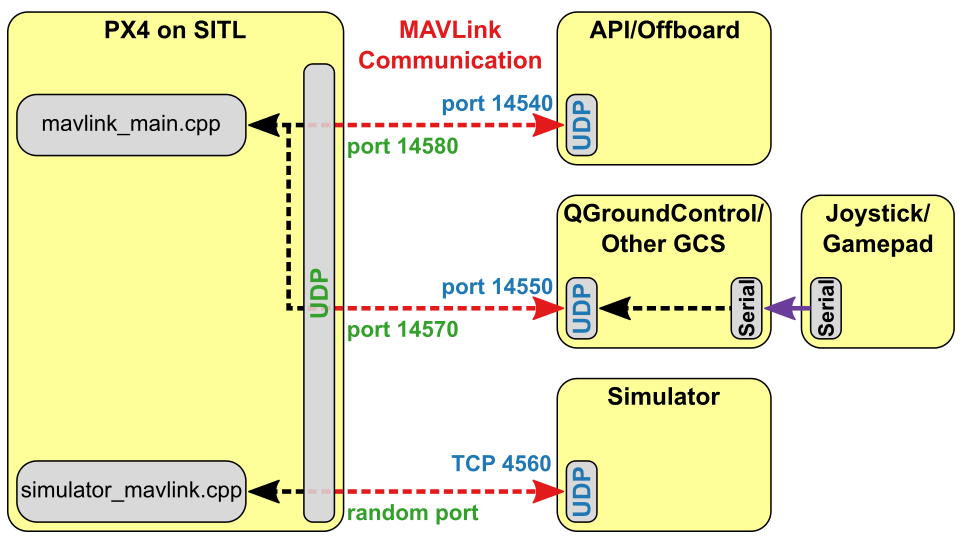
\includegraphics[width=0.8\textwidth]{picture/sitl.png}
    %   \caption{SITL}
    % \end{figure}
    % \begin{figure}[htbp]
    %   \centering
    %   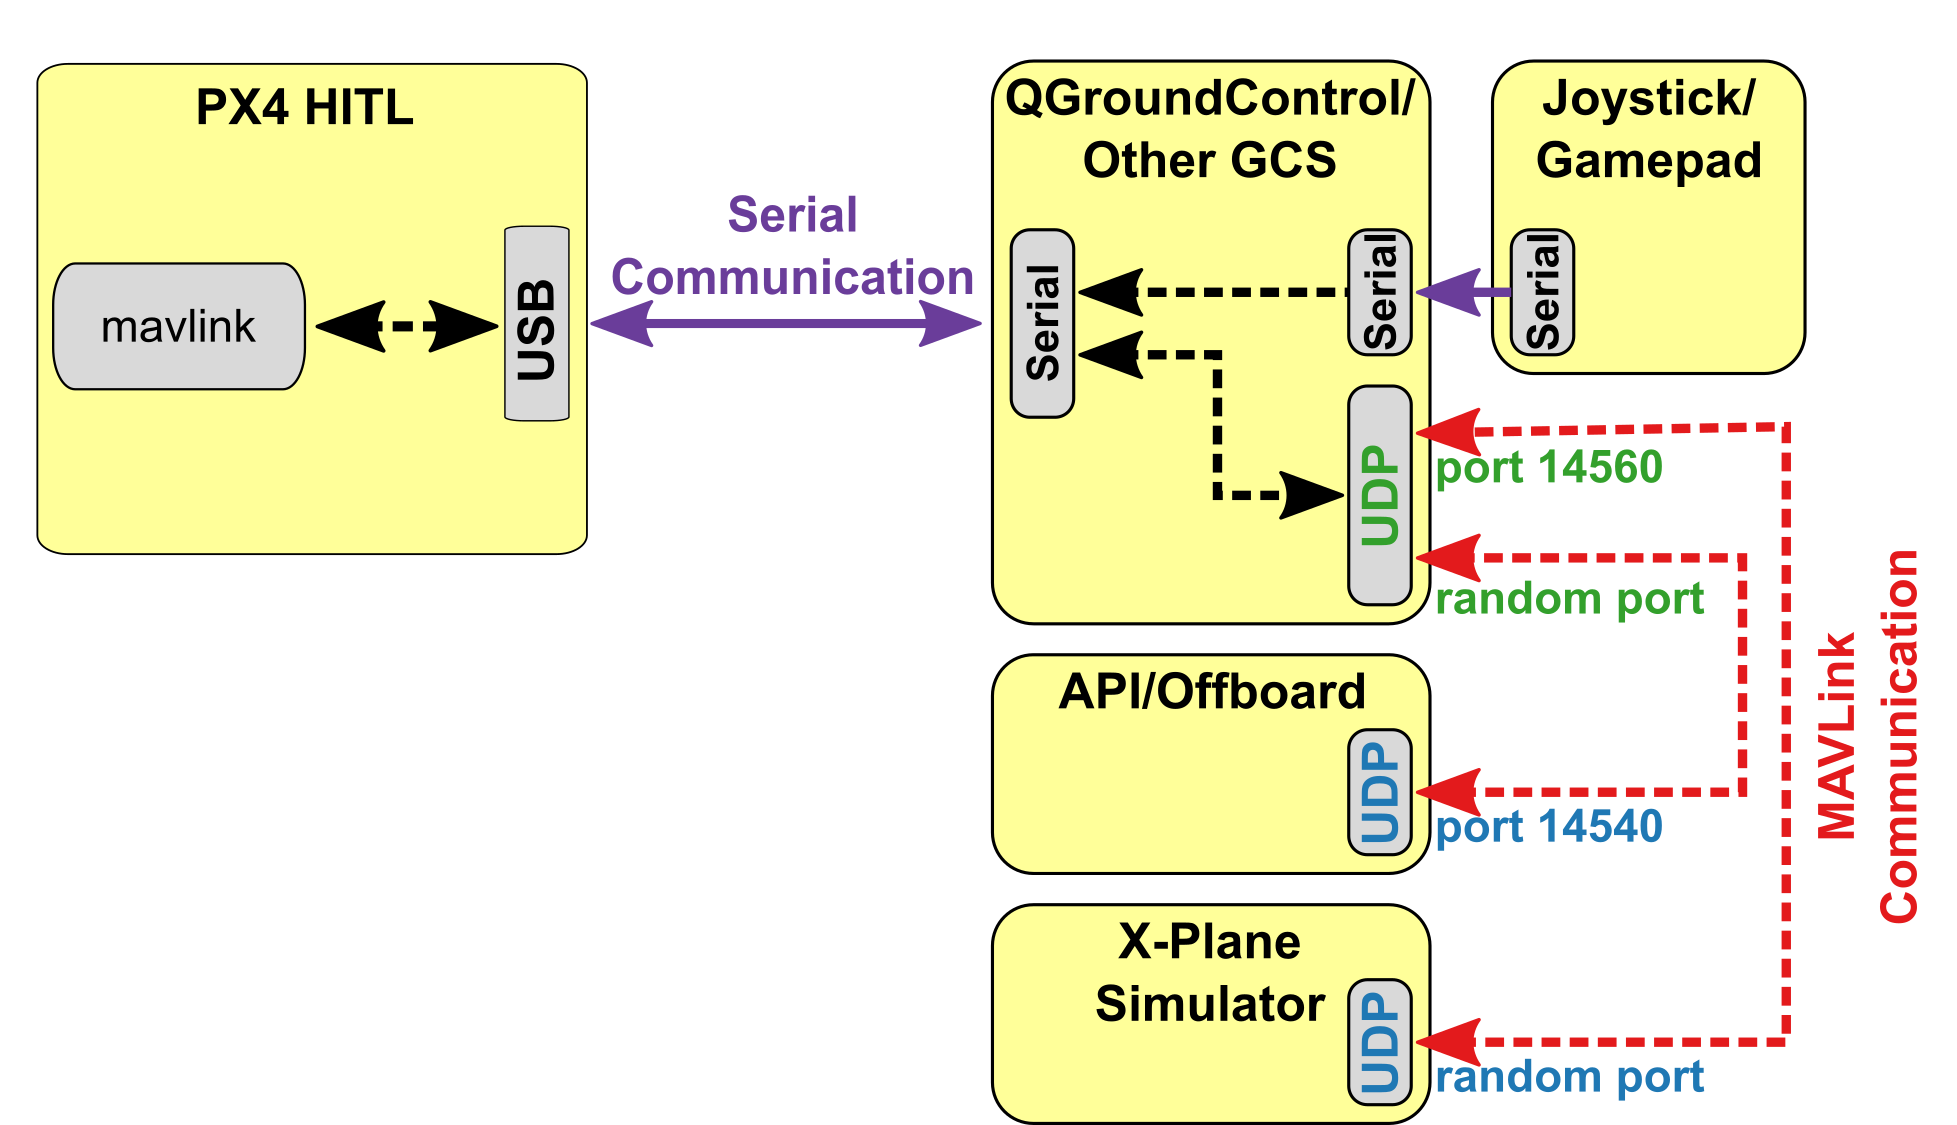
\includegraphics[width=0.8\textwidth]{picture/hitl.png}
    %   \caption{HITL-Xplane}
    % \end{figure}
    % \begin{figure}[htbp]
    %   \centering
    %   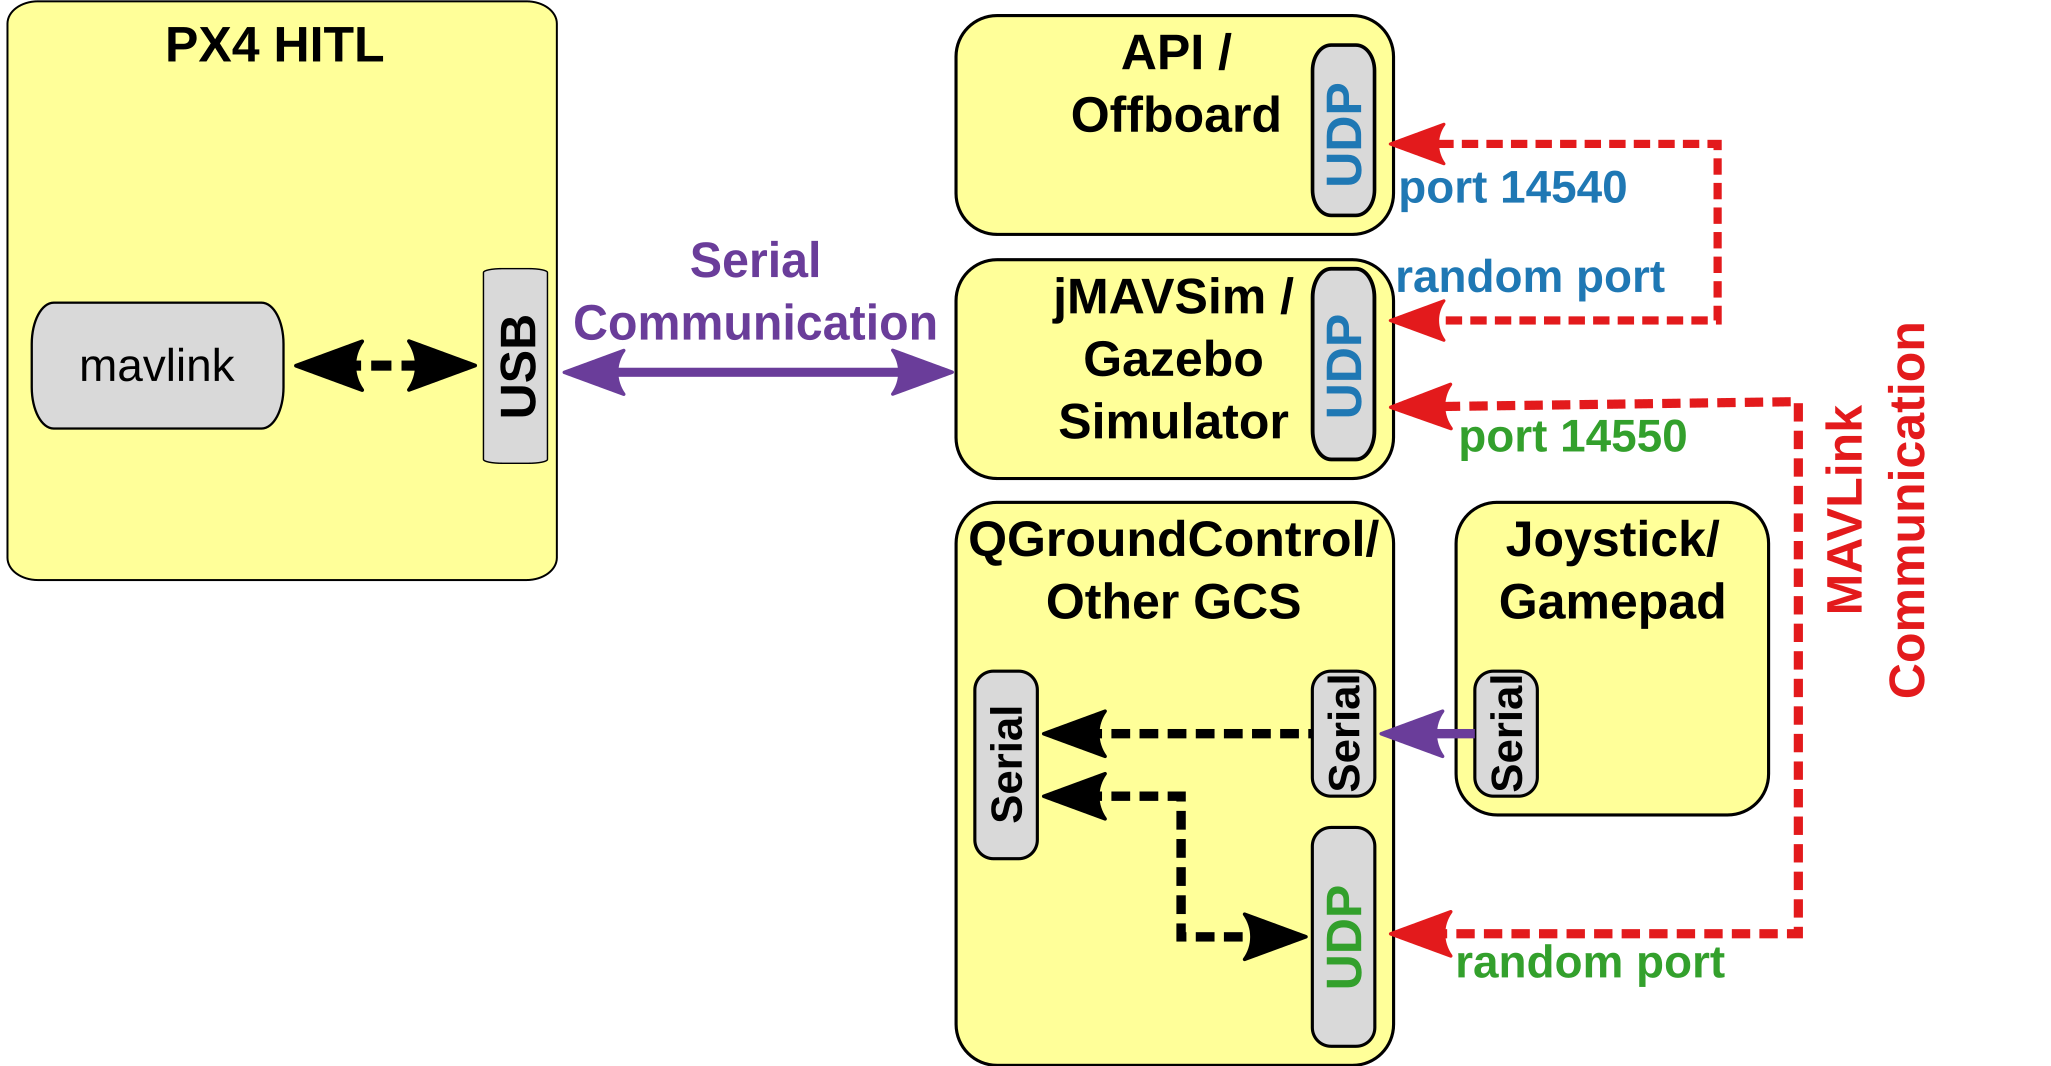
\includegraphics[width=0.8\textwidth]{picture/hitl2.png}
    %   \caption{HITL-Gazebo}
    % \end{figure}
    % \clearpage
    % \section{计算机视觉}
    %     整理一下当前的任务流.
    %   计算机视觉, 是一门研究如何对数字图像或视频进行高层语义理解的交叉学科, 赋予了机器"看"的能力, 需要实现人的大脑中(主要是视觉皮层区)的视觉能力. \par
    %   图像处理, 用计算机对图像进行分析, 已达到所需结果的技术. 图像处理一般指的是数字图像处理, 图像处理的技术一般包括图像压缩, 增强和复原, 匹配, 描述和识别三个部分. 
    %   \par 图像处理就是各种的图像变换处理, 计算机视觉在图像处理之后再识别其内部的语义, 理解视频流中的内容. 
    % \begin{figure}[htbp]
    %     \centering
    %     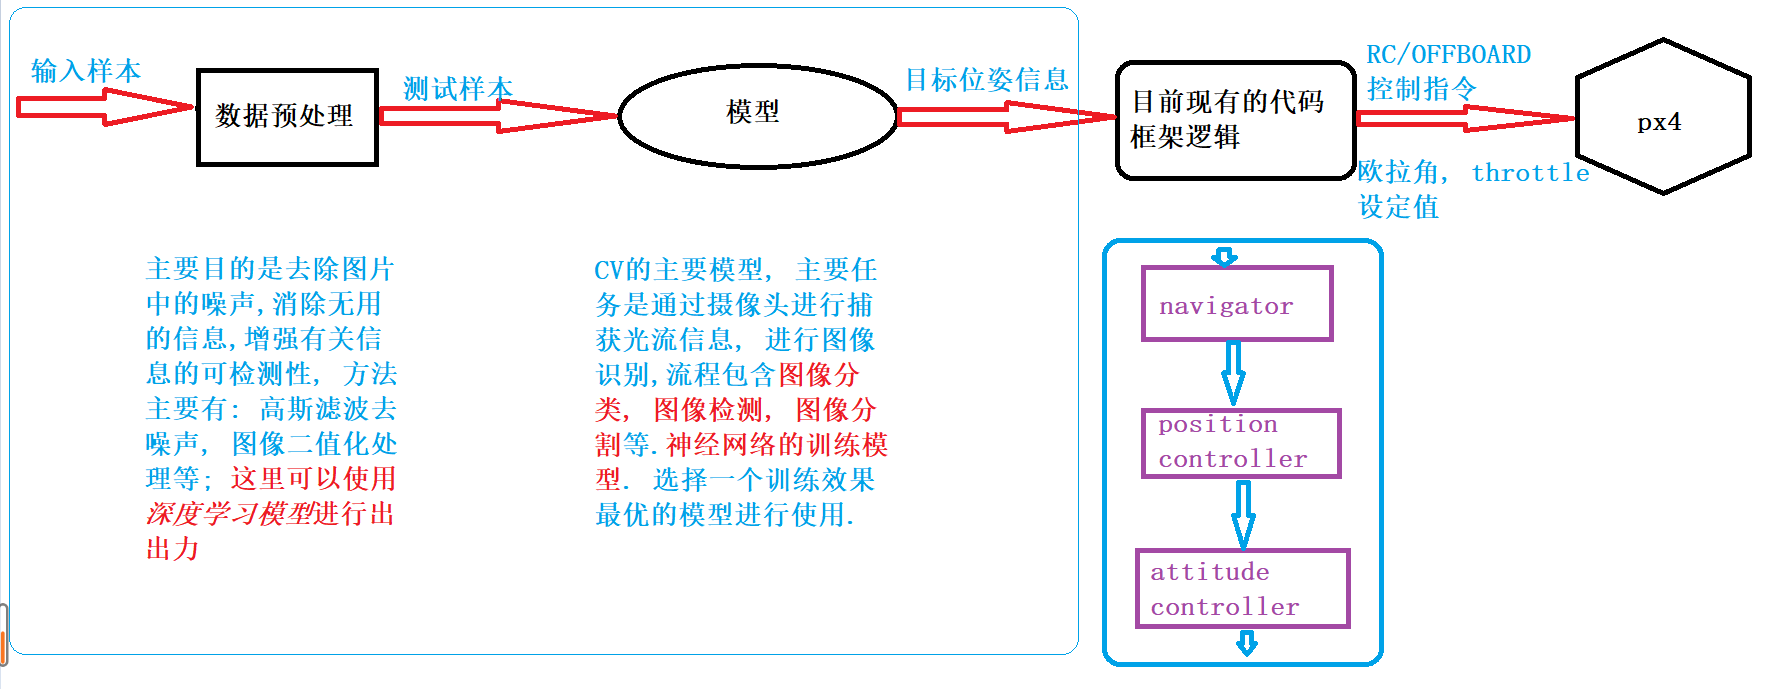
\includegraphics[width=0.8\textwidth]{picture/CV_Flow.png}
    %     \caption{CV数据流}
    % \end{figure}  
    % \clearpage
    % \section{算法内部}
    %     有时间的话细说一下代码
\end{document}

        \chapter{literature}
    \addcontentsline{toc}{section}{参考文献}
    \renewcommand{\refname}{参考文献}
    \begin{thebibliography}{99}
        \addtolength{\itemsep}{-2ex} % 用于更改行距
        \bibitem{1}杨玉,金敏,鲁华祥.融合简化稀疏A*算法与模拟退火算法的无人机航迹规划[J].计算机系统应用,2019,28(4):25-31. DOI:10.15888/j.cnki.csa.006864.
        \bibitem{2}张岳平,朱力超,孙涛.用Hopfield神经网络与模拟退火算法求解UAV航路规划问题[J].海军航空工程学院学报,2007,22(4):451-453,466. DOI:10.3969/j.issn.1673-1522.2007.04.012.
        \bibitem{3}赵梵喆,林跃,杨永琪.基于多目标规划的无人机路径规划[J].价值工程,2020,39(9):208-210.
        \bibitem{4}谭若晨.基于Multi-Agent系统的多UAV实时路径规划研究与实现[D].四川:电子科技大学,2013. DOI:10.7666/d.D772105.
        \bibitem{5}耿兴元.基于GPS与GIS的导航系统研究与开发[D].浙江:浙江大学,2004.
        \bibitem{6}张帅, 李学仁, 张鹏, 等.基于改进 A* 算法的无人机航迹规划[J] .飞行力学, 2016, 34( 3) : 39-43.
        \bibitem{7}Liu LF, Shi RX, Li SD, et al. Path planning for UAVS based
        on  improved  artificial  potential  field  method  through
        changing  the  repulsive  potential  function.  Proceedings  of
        2016  IEEE  Chinese  Guidance,  Navigation  and  Control
        Conference  (CGNCC).  Nanjing,  China.  2016.  2011–2015.
        \bibitem{8}D. R. Nelson, D. B. Barber, T. W. McLain and R. W. Beard, "Vector field path following for small unmanned air vehicles," 2006 American Control Conference, Minneapolis, MN, 2006, pp. 7 pp.-, doi: 10.1109/ACC.2006.1657648.
        \bibitem{9}Randal W. Beard and Timothy W. McLain, "Small Unmanned Aircraft: Theory and Practice", 2012, Princeton University Press
        \bibitem{10}R. W. {Beard} and T. W. {McLain} and D. B. {Nelson} and D. {Kingston} and D. {Johanson}, "Decentralized Cooperative Aerial Surveillance Using Fixed-Wing Miniature {UAVs}", 2006, Proceedings of the IEEE, 94, 7, 1306-1324
        \bibitem{11}R. W. {Beard} and J. {Ferrin} and J. {Humpherys}, "Fixed Wing {UAV} Path Following in Wind With Input Constraints", 2014, IEEE Transactions on Control Systems Technology, 2014, 22, 6, 2103-2117
        \bibitem{12}S. {Fari} and X. {Wang} and S. {Roy} and S. {Baldi}, "Addressing Unmodelled Path-Following Dynamics via Adaptive Vector Field: a {UAV} Test Case", 2019, IEEE Transactions on Aerospace and Electronic Systems, 10.1109/TAES.2019.2925487
    \end{thebibliography}  

\end{document}
